%Heterogeneous distributed GAs exploit the fact that with a sufficient number of processors, it is likely that at least some of the processors will end up being assigned a set of random control parameters which performs particularly well on a given problem. Therefore, the approach does not involve any meta- level learning or automated online parameter tuning. While numerous approaches to automated GA parameter configuration have been previously proposed, our naive method is attractive because of its simplicity. Although it is quite possible that a more sophisticated automated configuration methods could be adapted to perform well for a distributed GA, we believe that due to its extreme simplicity, the heterogeneous DGA proposed here can be considered a new baseline for evaluating more sophisticated approaches. \cite{gong2011distributed}

% Hacer un dibujito de pool-based model
% Abstract
% Leer todo
% Checar que tenemos font tipo 1 o eso
% Ver lo del double blind
% Checar siglas
% Checar constistencia: distributed, etc (leer para saber)
% Quitar el ACM Reference format (double blind):
% Homogeneizar el uso de italicas

\section{Introduction}
\label{introduction}

The particle swarm optimization (PSO) algorithm is an evolutionary algorithm (EA) distinguished by its suitability for optimization problems with continuous search spaces, in contrast to other EAs that are more suitable for combinatorial problems, such as genetic algorithms (GA). The reason behind this is that the population of solutions in the PSO algorithm (labeled as particles) move in the search space in a continuous manner, according to a direction dictated by the best particle or solution. As in the case of GA and other EA, PSO has a better possibility of converging to a solution if its population has high diversity (i.e. the particles are dispersed in the search space) \cite{morrison2001measurement}. In general, a bigger population in any EA should give solutions closer to the global minimum, but the algorithm will take more computational resources.

If a problem is sufficiently complex to require a relatively large number of particles in order to achieve a solution with a high fitness, the first and obvious solution is to increase the computational power available to the algorithm. Another solution, and one that has increased in popularity in the last decade, is to implement a distributed architecture. This kind of solutions usually partition the search space into a number of search sub-spaces equivalent to the number of devices participating in the distributed architecture \cite{sahin2007distributed}. A consequence of this approach is that several different instances of an EA will be running, one in each of the devices, and each of these instances can be configured with different values for their parameters. This could be seen as a drawback, as now one has to think on what parameters are the optimal for each device, or implement optimization algorithms to determine such values.

% got confused. parallel =! distributed
% explain that a device can be a physical device or a virtual device

Another problem arises with such distributed architectures: how are the populations going to be managed. One could only instruct each device to perform iterations (or \textit{generations}, using the EA jargon) using randomly generated solutions (or \textit{individuals}) in its corresponding search subspace, and after \textit{N} iterations the best solution is sent to the server \cite{sahin2007distributed}. Another solution is to follow the island-based model. % Add a reference
In this model, certain individuals are sent to the server,
% In the original island model, they are sent directly to other
% islands, this is the pool based approach.
and the server sends them to other devices and, therefore, to other search spaces. In other words, it can be said that individuals are traveling from one device (an \textit{island}) to another. The purpose of this technique is to influence the solutions of a particular search sub-space with a solution that was evolved in a different search sub-space, in hopes of making the architecture converge faster and avoid local minima.

A similar approach to the one taken in the island-based model is the pool-based % Here you are describing the EvoSpace model
model. In the pool-based model, every individual across every generation is controlled by the server. Devices in the parallel or distributed architecture extract a sample of individuals from the pool in the server. This sample is often determined randomly, as well as the size, although the size could be established in terms of the device's computational capacity, set to a fixed number, or determined by other factors. After the sample is gathered, it is sent to the device to be subjected to the evolutionary process, which can last for an arbitrary number of generations. If the EA finished successfully, the evolved sample is returned to the server pool (and if it fails, one of multiple processes can be performed, for example, the sample can be re-spawned in the server after a fixed amount of time, or the sample could get deleted). The individuals in the returned samples from each device can then be part of other samples that will be sent to another device. As a result, the major difference between the island-based model and the pool-based model is that the server can only examine those individuals who are migrating to other islands in the former, and the server can examine any individual at certain points in time during the evolutionary process in the latter \cite{garcia2014randomized}.

As mentioned before, a problem that arises when implementing an EA solution is determining the values of the different parameters of the algorithm. For example, in the case of the GA algorithm, one has to set the number of individuals in the initial population, what type of crossover methods are going to be used, the mutation and the crossover chance, to name some of the parameters. In order to determine the optimal values, several methods can be used, where choosing a value using one's experience would be the most simple of them. Another approach is to use another optimization algorithm, such as an EA, to tune the first EA, although this could result in an unsatisfying solution, because it adds another layer of parameters to be tuned. Instead of choosing a fixed set of values for the parameters of an EA, one can implement a controller that dynamically adapts the parameters' values according to some criteria. As an example, in the work by Melin et al. \cite{melin2013optimal},
% Justify why use this paper in your work
a fuzzy inference system is used as a controller to be changing the social and cognitive factors in the PSO, based on the current iteration the algorithm is at, the diversity of the particles, and the error among the particles. As can be noted, each of these methods (with the exception of the arbitrary selection of values) add an extra layer of complexity to the initial problem.

This work proposes the use of a randomized parameter setting (RPS) strategy to determine the values of the parameters in the PSO instances in a pool-based model. The benefit of implementing this strategy is that the aforementioned layer of complexity does not need to be added; all the parameters are set to random values, and implementing a parallel or distributed architecture for the pool-based model is already justified by its benefits in the increase of computational resources available for the optimization process. The drawback for this approach could be that setting the parameters in a randomly fashion is not going to be as effective as using a dynamic adapter, use another optimization method, or even set the parameters manually. This work presents a series of experiments that support the claim that the proposed method is as effective as a dynamic adapter, specifically a fuzzy inference system. %The hypothetical explanation for such results is that the PSO instances with randomized parameter settings help increase the position diversity of the particles, as each particle will participate in the evolutionary process of multiple PSOs.

% Mention the hypothesis of the increase of position diversity and the random parameter.

% Cambiar en el abstract por algo más como en este párrafo, además de considerar las sugerencias del doctor

A brief ee mentioned in Section \ref{conclusions}.xplanation of the other Sections in this paper follows. Section \ref{state-of-the-art} presents the state of the art in the area of parameter tuning with similar techniques described in the previous paragraphs. A series of related works are presented in Section \ref{related-work}, which are works that aim for the same goal as the present work, but propose different approaches to achieve it. Before describing the proposed method in Section \ref{proposed-method}, a series of preliminary concepts are explained in Section \ref{preliminaries}. The design of the experiments is presented in Section \ref{experiments}, and the results are discussed in Section \ref{results}. Finally, some conclusions are drawn and ar

\section{State of the Art}
\label{state-of-the-art}

The purpose of this Section is to provide the reader with a collection of works that demonstrate the current advances in the area of parameter tuning using RPS.

A work that uses RPS is the one by Gong and Fukunaga \cite{gong2011distributed}, where a genetic algorithm is tested using this strategy, in an island-based model and a distributed architecture. The authors state that the use of PSO can achieve good results for optimization purposes, but the algorithm is slow compared to other solutions.% Like what?
This serves as justification for implementing a distributed architecture that reduces the real time required to achieve the algorithm's goal. An issue that arises when designing such architecture is determining the values of the parameters for each PSO instance, but the authors decided to implement an RPS strategy yielding similar results to a homogeneous configuration among the devices in the distributed architecture (i.e. the values are established by hand, and every device runs with this configuration). Following the previously mentioned work, Tanabe and Fukunaga \cite{tanabe2013evaluation} continued experimenting with randomized parametrization in EAs with an island-based model. This work compares an heterogeneous randomization of parameters against manual tuning of parameters in differential evolution, an adaptive differential evolution, and in real-coded GAs. In the end, the authors found that randomized parametrization approaches the performance of the other strategies as the number of islands increases.

The work by Garcia-Valdez et al. \cite{garcia2014randomized} uses RPS for a GA, also using a pool-based model as in the present work. In order to prove the efficacy of their strategy, the authors compare RPS to three different parametrization strategies. The first parametrization strategy consists on a homogeneous setting: 200 random parameterizations are created, a GA runs each of these parameterizations, and an average of the runs is obtained. For the second strategy, the best configuration from the 200 random parameterizations is chosen, 20 more runs are performed with such configuration, and the average is obtained. Lastly, the third strategy consists on setting the parameters in a heterogeneous manner: every instance of a GA is initialized with randomized parameters, 20 runs are performed for this configuration and an average is obtained. In their results, it can be observed that using an heterogeneous parametrization can be as good as the other parametrization strategies.
%
% SoA is the same as Related Work ?
\section{Related Work}
\label{related-work}

A series of related works are presented in this Section. The main topics to be discussed are the implementation of distributed and parallel architectures in EAs, and the tuning of parameters in EAs using fuzzy inference systems (as the present work proposes the comparison of RPS against this particular strategy).

Merelo et al. have researched the area of distributed, pool-based and asynchronous techniques in EAs. As examples, \cite{merelo2008asynchronous} explores a distributed architecture constructed in Javascript, which leverages the capabilities of web browsers to run GAs. The results of this work show that the strategy is successful on reducing the time required by the GA to solve a problem as the number of devices participating in the evolutionary process increases (and it's also supported by their work in \cite{merelo2013designing}). Their method also supports the idea of implementing such architecture, as the devices participating in the process require almost no intervention from their users. In \cite{merelo2012pool}, Merelo et al. compare the island-based model against the pool-based model. This work supports the claim that a pool-based model usually has better scalability and will require less function evaluations in an EA than an island-based model, although the island-based model can sometimes perform faster than its counterpart.

Implementing a parallel architecture for an EA (i.e. several individuals are evaluated at the same time by multiple CPU or GPU cores \cite{mussi2011gpu}) can greatly increase its convergence speed, as can be seen in the work by McNabb et al. \cite{mcnabb2007parallel}, but this approach can be leveraged more by adopting an asynchronous model. As in the works by Koh et al. \cite{koh2006parallel} and Venter \cite{venter2006parallel}, one can send the individuals of the population in an EA to different CPU or GPU cores, without caring when these evaluated individuals will return to the central server. In a synchronous model, the server needs to wait for their evaluated individuals (or evolved individuals in the case that the devices performed an evolutionary process) to return, in order to determine what individuals will be sent to the participating devices for the next step in the process. In contrast, in an asynchronous architecture, the individuals are sent to other devices as soon as they arrive and are managed by the server, without needing for the other sample of individuals to return \cite{roy2009distributed}.

Lastly, the present work is related to the area of parameter tuning. The proposed method is compared to dynamic adaptation of parameters in EAs, in particular to the use of a fuzzy inference system to determine the values of the parameters. The work by Valdez et al. \cite{valdez2010fuzzy} demonstrates how to implement a fuzzy inference system that uses the current number of iterations in a GA to determine the mutation chance for that particular iteration. In a similar fashion, Melin et al. \cite{melin2013optimal} describe a set of fuzzy inference systems that control the cognitive and social factors in a PSO in terms of the number of iterations, and the diversity and error in the particles. Both of these works successfully increase the speed of convergence of their EAs by controlling how the algorithms enter the exploration and exploitation of solutions in their search spaces.

\section{Preliminaries}
\label{preliminaries}

Some preliminary concepts which are necessary to understand the proposed method in Section \ref{proposed-method} and the experiments in Section \ref{experiments} are explained in this Section.

\subsection{Pool-based Evolutionary Algorithms}

The basic idea behind pool-based EAs is that the population is gathered in a server (the \textit{pool}) and the evolutionary process is performed in another device. This device can be a \textit{virtual device}, which means that the evolutionary process is being performed on the same physical device, but it is logically separated from the pool server. This model facilitates implementing a parallel or a distributed architecture, as each of these virtual devices can be assigned to different threads in the CPU, different cores, different processors, or even different physical devices (distributed computing).

Both island and pool based EAs follow the previously mentioned idea. The difference between these two models lies in the role the server is going to perform. In the island-based model, the devices send individuals to the server to be migrated to other devices. The server receives these individuals and it determines the device it is going to send it to. In the pool-based model, the server is in charge of determining what individuals (or samples of the population) are going to be sent to each device, and all of these individuals are sent back to the server after certain criteria is met. As a consequence, in the island-based model the server can only interact with those individuals who are migrating to other devices, and in the pool-based model the server can interact with all the population at certain point.

\subsection{Fuzzy Inference Systems}
\label{fuzzy-inference-systems}

In a traditional set (or crisp set) an element either a member or not from that set. In contrast, in a fuzzy set \cite{zadeh1965fuzzy}, an element can have a grade of membership in that set. For example, an element that is \textit{somewhat} big can be a member of a "big elements" set, and also an element of a "medium-sized elements" set. Considering a fuzzy set, that element can have a grade of membership of 0.7 in the "big elements" set, and a grade of membership of 0.6 in the "medium-sized elements."

Fuzzy logic \cite{zadeh1988fuzzy} extends traditional logic by using fuzzy sets to describe the grade of \textit{truthfulness} of a fact. This way, one can obtain logical inferences by having a set of facts and rules that define how these facts are related. In the case of fuzzy logic, this kind of systems are called fuzzy inference systems (or fuzzy logic systems).

A fuzzy inference system defines a set of antecedents and a set of consequents. These antecedents and consequents can be defined by fuzzy sets (as in a Mamdani system \cite{mamdani1975experiment}) or by mathematical equations (as in a Takagi-Sugeno system \cite{takagi1985fuzzy}). The consequents will be activated or \textit{fired} depending on how truthful the antecedents are, and how were defined the fuzzy rules in the system. An example of a fuzzy rule would be "if the service is good, and the food quality is good, then the tip is high." In this case, \textit{service}, \textit{food quality} and \textit{tip} would be called linguistic variables, which are defined by a set of fuzzy sets, such as \textit{good}, \textit{bad}, \textit{low}, and \textit{high}.

\subsection{EvoSpace}
\label{evospace}

The EvoSpace platform \cite{garcia2013evospace} is used in the experiments of this work to implement a pool-based PSO. This platform is based on the tuple-space model, which is basically a repository that holds tuples of data. EvoSpace provides an interface to handle the tuple-space, i.e. functions to retrieve, insert, update, and delete tuples, as well as other more complex operations.

The platform was initially tested with interactive evolutionary computing problems, such as in \cite{garcia2013interactive}, but it has already been used to implement pool-based EAs \cite{garcia2015evospace}.

\section{Proposed Method}
\label{proposed-method}

The proposed method is designed to accelerate the convergence of the
PSO algorithm. The hypothesis that was taken into consideration for this method is
that extending PSO to a parallel architecture should increase the
position diversity of the particles, and avoid premature convergence around local optima and should yield better results because of this, as explained
by S. Cheng in \cite{cheng2013population}. Furthermore, each device in
the parallel architecture that is searching for a solution is configured with a
random set of parameters, as proposed by Y. Gong and A. Fukunaga in \cite{gong2011distributed}. This aproach, as \cite{gong2011distributed} expresses it, exploits the fact that with a sufficient number of instances of an EA, there is a high probability that one of the instances will have a set of randomized parameters that performs well on a given problem.

The PSO algorithm was adapted to be integrated with the EvoSpace
platform described in Section {evospace}. EvoSpace enables different
instances of PSO to be working on a single population, taking random
samples of particles, and updating the positions of these particles
according to the randomly determined cognitive and social factors set to each instance of the PSO algorithm. When a PSO instance requests a sample from the
population of particles, the best particle is also included in
the sample, i.e., the best particle considered is not the best in the
sample taken by the PSO instance, but the global best particle. This
ensures that all the PSO instances update the positions of its
samples' particles according to the global best.

All the PSO instances then proceed to update the sample particle
positions for a predetermined number of iterations. After the
iterations are completed, the sample is returned to the global
population in EvoSpace, and a new random sample is obtained by the PSO
instances that finished the evolutionary process and returned their
samples. This behaviour allows the PSO instances to update subsets of
particles of the population using different cognitive and social
factors.

As can be seen in Figure \ref{traditional-pso}, the particles in a
traditional PSO algorithm always move according to the best particle
(the red coloured particle, in this case) in each iteration, in terms
of the pre-established cognitive and
social factors. In contrast, one can see in Figure
\ref{distributed-pso} how the proposed method works. Each circled
group of particles have their positions updated in the plane according to the
social and cognitive factors of each PSO instance. In this case, each
circled group of particles represents a random sample of particles
taken from the population stored in EvoSpace. As was mentioned before,
this method should increase the diversity of the particles in the
population, and the randomized parameter setting should help particles
converge to a solution as fast as a PSO with dynamic adaptation of its
parameters.

\begin{figure}
  \centering
  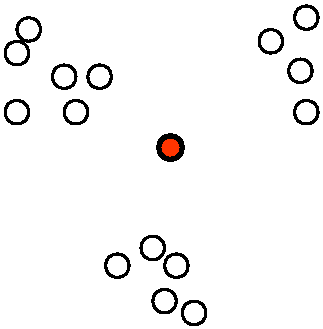
\includegraphics[height=4cm]{pdf/traditional-pso}
  \caption{}
  \label{traditional-pso}
\end{figure}

\begin{figure}
  \centering
  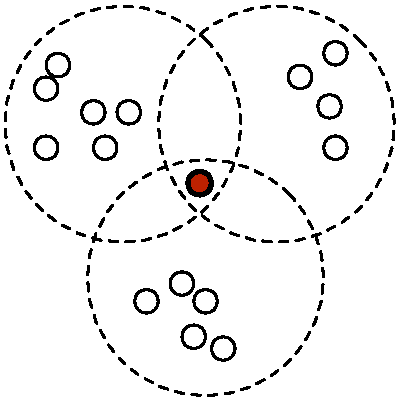
\includegraphics[height=4cm]{pdf/distributed-pso}
  \caption{}
  \label{distributed-pso}
\end{figure}

Lastly, the proposed method enables different physical devices to get
involved in the evolutionary process. A device can request a sample of
the particles and it updates their positions for a certain number of
generations. After finishing this process, the device returns the
updated sample to the EvoSpace server. This architecture allows the
physical devices to work asynchronously and in parallel.

\section{Experiments}
\label{experiments}

In order to compare the proposed method presented in Section \ref{proposed-method}, a set of other parameter tuning strategies were defined. These strategies are based on the ones presented in the work by Melin et al. \cite{melin2013optimal}, where a dynamic adaptation of the cognitive and the social factors in the particle swarm optimization algorithm is performed using a fuzzy inference system (this kind of systems are explained in Section \ref{fuzzy-inference-systems}). The authors of the aforementioned work propose three different dynamic adaptation of parameters strategies: 1) a fuzzy inference system takes as inputs the current number of iterations and the diversity of the particles, and give as output the social and cognitive factors; 2) a fuzzy inference system takes as inputs the current number of iterations and the error among the particles, and give as output the social and cognitive factors; and 3) a fuzzy inference system takes as inputs the current number of iterations, the diversity of the particles, and the error among the particles, and give as output the social and cognitive factors.

The objective of the work in \cite{melin2013optimal} was to determine what combination of inputs was better to perform a dynamic adaptation of parameters in a PSO. In the case of the present work, the authors propose that a randomized parameterization will achieve better or similar results than any of the proposed strategies in \cite{melin2013optimal}, supporting the idea that a good parameter tuning in EAs can be achieved by randomized parameterization.

In order to give shorter descriptions of the dynamic adaptation strategies, it can be mentioned that all of the membership functions (the fuzzy sets that describe an adjective of an antecedent or a consequent) are described by triangular functions. For a triangular membership function, one has to define three points (\textit{a}, \textit{b}, and \textit{c}), where $f(a) = 0$, $f(b) = 1$, $f(c) = 0$, and $a <= b <= c$. The social and the cognitive factors, represented by $c1$ and $c2$, range in domain from 0 to 3, as values in this interval are recommended in the literature \cite{kenndy1995particle}. The rule bases for the strategies are obtained from \cite{melin2013optimal}.

The first strategy, called Fuzzy PSO 1, is configured as follows. The first antecedent, \textit{iterations}, has a domain from 0 to 1, which represents the percentage of iterations completed at a certain point, and is described by three adjectives: low, medium, and high. In the case of \textit{low}, $a = 0$, $b = 0$, and $c = 0.5$; for \textit{medium}, $a = 0$, $b = 0.5$, and $c = 1$; and for \textit{high}, $a = 0.5$, $b = 1$, and $c = 1$. The second antecedent, \textit{diversity}, has a domain from 0 to 1, and is described by three adjectives: low, medium, and high. In the case of \textit{low}, $a = 0$, $b = 0$, and $c = 0.5$; for \textit{medium}, $a = 0$, $b = 0.5$, and $c = 1$; and for \textit{high}, $a = 0.5$, $b = 1$, and $c = 1$. For the consequents, \textit{c1} and \textbf{c2}, both have a domain from 0 to 3, and are described by five adjectives each: low, medium-low, medium, medium-high and high. In the case of \textit{low}, $a = 0$, $b = 0.5$, and $c = 1$; for \textit{medium-low}, $a = 0.5$, $b = 1$, and $c = 1.5$; for \textit{medium}, $a = 1$, $b = 1.5$, and $c = 2$; for \textit{medium-high}, $a = 1.5$, $b = 2$, and $c = 2.5$; lastly, for \textit{high}, $a = 2$, $b = 2.5$, and $c = 3$.

The second strategy, called Fuzzy PSO 2, is similar than Fuzzy PSO 1, with a slight difference in the antecedents. Instead of \textit{iterations} and \textit{diversity}, it uses \textit{iterations} and \textit{error}. This antecedent, \textit{error}, has a domain from 0 to 1, and is described by three adjectives: low, medium, and high. In the case of \textit{low}, $a = 0$, $b = 0$, and $c = 0.5$; for \textit{medium}, $a = 0$, $b = 0.5$, and $c = 1$; and for \textit{high}, $a = 0.5$, $b = 1$, and $c = 1$. The remaining antecedent and consequents are described the same way as in Fuzzy PSO 1.

For the third strategy, called Fuzzy PSO 3, \textit{iterations}, \textit{diversity} and \textit{error} are considered as antecedents, and \textit{c1} and \textit{c2} as the consequents. All of them are defined the same as in Fuzzy PSO 1 and Fuzzy PSO 2.



In the case of the proposed method, five instances of PSO are created, which are going to be drawing individuals from the population in the server pool. Every time an instance obtains a new sample of individuals, it performs an evolutionary process of only one generation, using randomized values for \textit{c1} and \textit{c2}. The sample size will be $N/5$, meaning that each device will have an equally sized sample. The samples always gather the individuals by random choice.

For each of the strategies mentioned in this Section, an initial population of 200 individuals is randomly generated, and they will be evolved for 100 iterations. The objective for these strategies is to obtain the global minimum for the following benchmark functions: Sphere, Ackley, Rastrigin, Griewank, and Schaffer (number 2).

While the strategies run, the diversity in position of the particles is recorded in every iteration. In addition to diversity, interest is given to the number of evaluations required for each method to reach certain threshold of error. In order to avoid converging to said threshold too soon or too late, a simple PSO with $c1 = 1$ and $c2 = 3$ is run 100 times, and the error obtained by the 90th percentile is used as the threshold. The reason behind this is that if a very low threshold is used, the strategies could never converge to it, and every strategy would report similar number of evaluations. Likewise, if a very high threshold is used, the strategies could converge to it too early, and every strategy would also report similar number of evaluations.

% Rule base for three methods
% Membership functions for three methods

\section{Results}
\label{results}

This Section presents the results of implementing the concepts discussed in Sections \ref{proposed-method} and \ref{experiments}. The basic procedure is to perform comparisons between each strategy against the proposed method, called PB-RPS PSO (pool-based randomized parameter settings PSO) in the results tables. These comparisons take into consideration the diversity of the particles in each iteration, and the number of evaluations, obtained as is explained in Section \ref{experiments}. For these comparisons, five benchmark functions are used: Sphere, Ackley, Rastrigin, Griewank, and Schaffer (number 2).

For the comparisons in terms of number of evaluations, 100 runs of each strategy are performed, and the number of evaluations is recorded after each run. The average and standard deviations are calculated and used to perform hypothesis tests. In the case of the comparisons in terms of diversity, 30 runs of each strategy are performed, for 100 generations. After each generation finishes its evolutionary process, the diversity in the particles is recorded, giving as result a record of 100 diversities for each of the 30 runs. In order to obtain the final averages and standard deviations for each strategy, the average and standard deviation of the 100 generations is calculated for each of the 30 runs, and the average is calculated for these 30 averages and 30 standard deviations, and they are used to perform hypothesis tests.

For the diversity comparisons, the hypothesis tests are considering that the proposed method obtains a higher diversity in its population. In the case of the number of evaluations, what is being considered is that the proposed method obtains a lower number than the other strategies. The results tables show t-Values and confidence intervals to illustrate how well the proposed method performed against the corresponding strategy. If a hyphen is printed instead of a confidence interval, this means that the proposed method performed similarly than the corresponding strategy (a t-Value corresponding to a confidence interval of less than 80\% was calculated).

In the case of the Sphere benchmark function, Tables \ref{evaluations-sphere} and \ref{diversity-sphere} show the results for the evaluations and diversity comparisons, respectively. For this function, the proposed method outperforms the other strategies with very high confidence intervals.

\begin{table}[!t]
  \renewcommand{\arraystretch}{1.3}
  \caption{Comparison of Number of Evaluations for Each Method Using the Sphere Function Benchmark}
  \label{evaluations-sphere}
  \centering
  \begin{tabular}{|c|c|c|c|c|c|}
    \hline
    Method & $\mu$ & $SD$ & $n$ & t-Value & CI \\
    \hline
    PSO 		& 43006.68 & 54068.88 & 100 & 5.5824 & $>$ 99.9\% \\
    \hline
    Fuzzy PSO 1 & 26229.81 & 32227.98 & 100 & 4.0730  & $>$ 99.9\% \\
    \hline
    Fuzzy PSO 2 & 29120.29 & 34616.94 & 100 & 4.5943 & $>$ 99.9\% \\
    \hline
    Fuzzy PSO 3 & 22579.79 & 29345.82 & 100 & 3.3072 & $>$ 99.8\% \\
    \hline
    PB-RPS PSO  & 11192.68 & 18009.82 & 100 &  &  \\
    \hline
  \end{tabular}
\end{table}
% Critical t 99.8% 3.140569, Critical t 99.9% 3.350726

\begin{table}[!t]
  \renewcommand{\arraystretch}{1.3}
  \caption{Comparison of Diversity in Particles for Each Method Using the Sphere Function Benchmark}
  \label{diversity-sphere}
  \centering
  \begin{tabular}{|c|c|c|c|c|c|}
    \hline
    Method & $\mu$ & $SD$ & $n$ & t-Value & CI \\
    \hline
    PSO 		& 0.669875 & 0.122061 & 30 & 4.8351 & $>$ 99.9\% \\
    \hline
    Fuzzy PSO 1 & 0.699300 & 0.102249 & 30 & 4.1872 & $>$ 99.9\% \\
    \hline
    Fuzzy PSO 2 & 0.698955 & 0.108778 & 30 & 4.0010 & $>$ 99.9\% \\
    \hline
    Fuzzy PSO 3 & 0.715489 & 0.091104 & 30 & 3.7341 & $>$ 99.9\% \\
    \hline
    PB-RPS PSO  & 0.787360 & 0.053044 & 30 &  &  \\
    \hline
  \end{tabular}
\end{table}
% Critical t 99.8% 3.140569, Critical t 99.9% 3.350726

The second benchmark function used is Ackley. Tables \ref{evaluations-ackley} and \ref{diversity-ackley} show these results. Regarding the number of evaluations, the proposed method performed similarly against every strategy, except a traditional PSO without parameter tuning. In the case of the diversity comparisons, the proposed method outperformed every strategy.

\begin{table}[!t]
  \renewcommand{\arraystretch}{1.3}
  \caption{Comparison of Number of Evaluations for Each Method Using the Ackley Function Benchmark}
  \label{evaluations-ackley}
  \centering
  \begin{tabular}{|c|c|c|c|c|c|}
    \hline
    Method & $\mu$ & $SD$ & $n$ & t-Value & CI \\
    \hline
    PSO 		& 3617.62 & 6150.64 & 100 & 2.2259 & $>$ 97\% \\
    \hline
    Fuzzy PSO 1 & 2175.09 & 4343.38 & 100 & 0.2316 & - \\
    \hline
    Fuzzy PSO 2 & 2468.17 & 4603.34 & 100 & 0.7321 & - \\
    \hline
    Fuzzy PSO 3 & 2052.17 & 3815.28 & 100 & 0.0111 & - \\
    \hline
    PB-RPS PSO  & 2046.45 & 3462.85 & 100 &  &  \\
    \hline
  \end{tabular}
\end{table}
% Critical t 97% 2.190116
% Critical t 99.8% 3.140569,
%Critical t 99.9% 3.350726

\begin{table}[!t]
  \renewcommand{\arraystretch}{1.3}
  \caption{Comparison of Diversity in Particles for Each Method Using the Ackley Function Benchmark}
  \label{diversity-ackley}
  \centering
  \begin{tabular}{|c|c|c|c|c|c|}
    \hline
    Method & $\mu$ & $SD$ & $n$ & t-Value & CI \\
    \hline
    PSO 		& 0.671121 & 0.120527 & 30 & 4.5643 & $>$ 99.9\% \\
    \hline
    Fuzzy PSO 1 & 0.703941 & 0.103029 & 30 & 3.6422 & $>$ 99.9\% \\
    \hline
    Fuzzy PSO 2 & 0.701419 & 0.103141 & 30 & 3.7562 & $>$ 99.9\% \\
    \hline
    Fuzzy PSO 3 & 0.709849 & 0.092386 & 30 & 3.6519 & $>$ 99.9\% \\
    \hline
    PB-RPS PSO  & 0.782361 & 0.057382 & 30 &  &  \\
    \hline
  \end{tabular}
\end{table}
% Critical t 99.8% 3.140569, Critical t 99.9% 3.350726



Tables \ref{evaluations-rastrigin} and \ref{diversity-rastrigin} show the results for the Rastrigin benchmark function. The proposed method performed similarly in the cases of Fuzzy PSO 1 and Fuzzy PSO 2, but outperformed Fuzzy PSO 1 with a confidence interval of 90\%. In the case of diversity comparisons, the proposed method outperformed the other strategies.


\begin{table}[!t]
  \renewcommand{\arraystretch}{1.3}
  \caption{Comparison of Number of Evaluations for Each Method Using the Rastrigin Function Benchmark}
  \label{evaluations-rastrigin}
  \centering
  \begin{tabular}{|c|c|c|c|c|c|}
    \hline
    Method & $\mu$ & $SD$ & $n$ & t-Value & CI \\
    \hline
    PSO 		& 4585.93 & 6756.02 & 100 & 3.3529 & $>$ 99.8\% \\
    \hline
    Fuzzy PSO 1 & 3148.97 & 5625.51 & 100 & 1.6683 & $>$ 90\% \\
    \hline
    Fuzzy PSO 2 & 2332.24 & 4056.50 & 100 & 0.5252 & - \\
    \hline
    Fuzzy PSO 3 & 2648.31 & 4808.98 & 100 & 1.0102 & - \\
    \hline
    PB-RPS PSO  & 2055.44 & 3363.98 & 100 &  &  \\
    \hline
  \end{tabular}
\end{table}
% Critical t 99.8% 3.140569, Critical t 99.9% 3.350726
% Critical t 90.0% 1.654326

\begin{table}[!t]
  \renewcommand{\arraystretch}{1.3}
  \caption{Comparison of Diversity in Particles for Each Method Using the Rastrigin Function Benchmark}
  \label{diversity-rastrigin}
  \centering
  \begin{tabular}{|c|c|c|c|c|c|}
    \hline
    Method & $\mu$ & $SD$ & $n$ & t-Value & CI \\
    \hline
    PSO 		& 0.651842 & 0.128705 & 30 & 2.3541 & $>$ 97\% \\
    \hline
    Fuzzy PSO 1 & 0.664845 & 0.104125 & 30 & 2.1769 & $>$ 96\% \\
    \hline
    Fuzzy PSO 2 & 0.671310 & 0.104255 & 30 & 1.9010 & $>$ 93\% \\
    \hline
    Fuzzy PSO 3 & 0.671683 & 0.099991 & 30 & 1.9364 & $>$ 94\% \\
    \hline
    PB-RPS PSO  & 0.716133 & 0.076222 & 30 &  &  \\
    \hline
  \end{tabular}
\end{table}
% Critical t 99.8% 3.140569, Critical t 99.9% 3.350726
% Critical t 97% 2.237803
% Critical t 96% 2.10539
% Critical t 94% 1.920986

For the Griewank benchmark function, Tables \ref{evaluations-griewank} and \ref{diversity-griewank} show the results. The proposed method could not outperform any of the other strategies regarding the number of evaluations, but obtained a higher diversity.

\begin{table}[!t]
  \renewcommand{\arraystretch}{1.3}
  \caption{Comparison of Number of Evaluations for Each Method Using the Griewank Function Benchmark}
  \label{evaluations-griewank}
  \centering
  \begin{tabular}{|c|c|c|c|c|c|}
    \hline
    Method & $\mu$ & $SD$ & $n$ & t-Value & CI \\
    \hline
    PSO 		& 2721.55 & 5664.44 & 100 & 2.3198 & $>$ 97\% \\
    \hline
    Fuzzy PSO 1 & 983.02 & 2387.89 & 100 & -0.7227 & - \\
    \hline
    Fuzzy PSO 2 & 1430.06 & 3424.02 & 100 & 0.4017 & - \\
    \hline
    Fuzzy PSO 3 & 1602.23 & 3720.41 & 100 & 0.7495 & - \\
    \hline
    PB-RPS PSO  & 1251.31 & 2842.61 & 100 &  &  \\
    \hline
  \end{tabular}
\end{table}
% Critical t 99.8% 3.140569, Critical t 99.9% 3.350726

\begin{table}[!t]
  \renewcommand{\arraystretch}{1.3}
  \caption{Comparison of Diversity in Particles for Each Method Using the Griewank Function Benchmark}
  \label{diversity-griewank}
  \centering
  \begin{tabular}{|c|c|c|c|c|c|}
    \hline
    Method & $\mu$ & $SD$ & $n$ & t-Value & CI \\
    \hline
    PSO 		& 0.517035 & 0.175668 & 30 & 5.8144 & $>$ 99.9\% \\
    \hline
    Fuzzy PSO 1 & 0.543398 & 0.150292 & 30 & 5.7503 & $>$ 99.9\% \\
    \hline
    Fuzzy PSO 2 & 0.535249 & 0.154780 & 30 & 5.8752 & $>$ 99.9\% \\
    \hline
    Fuzzy PSO 3 & 0.558314 & 0.147237 & 30 & 5.3518 & $>$ 99.9\% \\
    \hline
    PB-RPS PSO  & 0.720288 & 0.076162 & 30 &  &  \\
    \hline
  \end{tabular}
\end{table}
% Critical t 99.8% 3.140569, Critical t 99.9% 3.350726

Lastly, the Schaffer benchmark function proved to be the most difficult for the proposed method, as it could not even outperform a traditional PSO without parameter tuning in terms of diversity. Furthermore, in terms of number of evaluations, the Fuzzy PSO 1 strategy outperformed the proposed method. Tables \ref{evaluations-schaffer} and \ref{diversity-schaffer} show these results.

\begin{table}[!t]
  \renewcommand{\arraystretch}{1.3}
  \caption{Comparison of Number of Evaluations for Each Method Using the Schaffer Function Benchmark}
  \label{evaluations-schaffer}
  \centering
  \begin{tabular}{|c|c|c|c|c|c|}
    \hline
    Method & $\mu$ & $SD$ & $n$ & t-Value & CI \\
    \hline
    PSO 		& 1130.14 & 3332.44 & 100 & 1.0448 & $>$ 99.9\% \\
    \hline
    Fuzzy PSO 1 & 257.24 & 103.88 & 100 & -3.0081 & \textbf{$>$ 99.6\%*} \\
    \hline
    Fuzzy PSO 2 & 719.46 & 2029.19 & 100 & -0.0921 & - \\
    \hline
    Fuzzy PSO 3 & 531.15 & 921.20 & 100 & -1.1425 & - \\
    \hline
    PB-RPS PSO  & 743.34 & 1612.64 & 100 &  &  \\
    \hline
  \end{tabular}
\end{table}
% Critical t 99.8% 3.140569, Critical t 99.9% 3.350726
% Critical t 99.6% 2.946542

\begin{table}[!t]
  \renewcommand{\arraystretch}{1.3}
  \caption{Comparison of Diversity in Particles for Each Method Using the Schaffer Function Benchmark}
  \label{diversity-schaffer}
  \centering
  \begin{tabular}{|c|c|c|c|c|c|}
    \hline
    Method & $\mu$ & $SD$ & $n$ & t-Value & CI \\
    \hline
    PSO 		& 0.577959 & 0.154588 & 30 & 1.5949 & - \\
    \hline
    Fuzzy PSO 1 & 0.621907 & 0.125628 & 30 & 0.4059 & - \\
    \hline
    Fuzzy PSO 2 & 0.633739 & 0.106091 & 30 & 0.0336 & - \\
    \hline
    Fuzzy PSO 3 & 0.614831 & 0.132162 & 30 & 0.6131 & - \\
    \hline
    PB-RPS PSO  & 0.634716 & 0.118723 & 30 &  &  \\
    \hline
  \end{tabular}
\end{table}
% Critical t 99.8% 3.140569, Critical t 99.9% 3.350726


\section{Conclusions}
\label{conclusions}

The results obtained in this work support the use of randomized parameterization in the particle swarm optimization algorithm when used in a pool-based model. The use of a strategy for parameter tuning should not be necessary for several optimization problems if using the strategy described in the proposed method.

A high diversity in the particles should help the algorithm to not fall into local minima prematurely, and a low number of evaluations means less computational power is needed in order to obtain satisfactory results. Furthermore, the high diversity could be the reason for the high convergence rate of the proposed method, but this hypothesis would need a different set of experiments to be proved.
